Los modelos de redes neuronales artificiales, uno de los cuales es el
\textit{perceptrón} que discutiremos en este capitulo, están
inspirados en el cerebro humano. Hay científicos cognitivos y de
neurociencia cuya meta es entender el funcionamiento del cerebro, y
con esto en mente, construir modelos de las redes neuronales naturales
del cerebro.

Sin embargo, lo que busca la inteligencia artificial es construir
máquinas \textit{útiles} tomando como modelo el cerebro. El cerebro es
un dispositivo de procesamiento de información con habilidades
asombrosas en muchos campos que sobrepasan con creces a los más
grandes esfuerzos de la ingenieria, como son visión, aprendizaje y
reconocimiento del habla, por nombrar algunos.

\section{Inspiracion en la biología}
El cerebro humano es muy diferente de una computadora. Mientras una
computadora tiene un número reducido de procesadores, el cerebro está
compuesto de una enorme cantidad $(10^{11})$ de unidades de
procesamiento llamadas \textbf{neuronas} trabajando en paralelo.

Aunque los detalles son inciertos, se cree que las neuronas son mucho
más simples y lentas que un procesador de una computadora
\cite{ethem}. Lo que hace al cerebro distinto, y le da su gran poder
computacional, es su gran conectividad: las neuronas en el cerebro
tienen conexiones, llamadas \textit{sinápsis}, a alrededor de otras
$10^{4}$ neuronas.

En una computadora, el procesador es activo y la memoria está separada
operando de forma pasiva (el procesador accede a ella sólo cuando se
requiere); se cree que en el cerebro, tanto el procesamiento como la
memoria están distribuidos por toda la red. El procesamiento es
realizado por las neuronas y la memoria se encuentra en las sinápsis
entre ellas.

El cerebro es, además, un órgano capás de adaptarse a las condiciones
de su ambiente, ya que constantemente son agregadas nuevas conexiones
sinápticas entre neuronas y modificadas las ya existentes. Una vez que
una neurona ha emitido una señal eléctrica, las adyacentes reciben la
información por medio de canales de transmisión llamados
\textit{dendritas}. Estos impulsos son llevados hasta el
\textit{núcleo} de la neurona para su procesamiento y, posteriormente,
una reacción es transmitida a través del \textit{axón} de la célula
\cite{memes}.
\begin{figure}[h]
  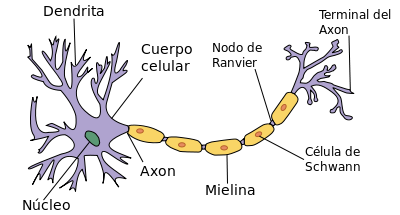
\includegraphics{neurona} \centering
  \caption{Estructura de una neurona. (Tomado de
    \url{https://es.wikipedia.org/wiki/Neurona})}
\end{figure}

\section{El perceptrón}
En 1943, Warren McCullock y Walter Pitts publican la primera
aproximación de una neurona simplificada, tratando de entender cómo
funciona el cerebro biológico para el diseño de inteligencia
artificial, la llamada neurona McCullock-Pits (MCP) \cite{mcp}.

McCullock y Pitts describen a la neurona como una compuerta lógica
sencilla con una salida binaria; múltiples señales llegan a las
dendritas para ser integradas al cuerpo de la célula. Si la señal
acumulada excede cierto umbral, se genera una señal de salida que se
le pasa al axón.

Unos años después, Frank Rosenblatt publica la primera aproximación al
concepto de perceptron basado en el modelo de neuronas MCP
\cite{rosenblatt}. Intuitivamente, el algoritmo aprende
automáticamente los coeficientes de pesos óptimos que luego se
multiplican con las características de entrada para tomar la decisión
de si la neurona se activa o no. Este algoritmo podría ser usado
entonces para predecir si una muestra pertenece a una clase o a otra
\cite{python}.

Formalmente, podemos plantearlo como un problema de clasificación
binaria, donde nos referimos a nuestras dos clases, por simplicidad,
como 1 (clase positiva) y -1 (clase negativa). Definimos también una
\textit{función de activación $\mathbf{\phi (z)}$} que toma una
combinación lineal de ciertos valores de entrada \textbf{x} y un
vector de pesos \textbf{w}, donde \textbf{z} es lo que llamamos
\textit{entrada de la red} $(z = w_1x_1 + ... + w_mx_m)$:

\begin{equation*}
w=
    \begin{bmatrix}
        w_1 \\ \vdots \\ w_m
    \end{bmatrix}
    , x=
    \begin{bmatrix}
      x_1 \\ \vdots \\ x_m
    \end{bmatrix}
\end{equation*}
\\ Si la activación de una muestra particular $x^{(i)}$ es mayor que
un parámetro definido $\theta$, predecimos la clase 1, y la clase -1
en caso contrario. En el algoritmo del perceptrón de Rosenblatt, la
activación de función $\phi (\dot)$ es una \textit{función escalón},
que es llamada a veces la \textit{función de Heaviside}:
\begin{equation*}
  \phi(z)= \left\{ \begin{array} {rl} 1 & \text{si } z \geq \theta
    \\ -1 & \text{en otro caso} \end{array} \right.
\end{equation*}

Por simplicidad, definimos $w_0=-\theta$ y $x_0=1$, escribiendo
entonces a $z$ de la forma $z=w_0x_0 + w_1x_1 + \dots + w_mx_m =
\mathbf{w^Tx}$.  La figura \ref{fig:binary} ilustra cómo la entrada de
la red $z=w^Tx$ es \textit{aplanada} a una salida binaria (-1 o 1) por
la función de activación del perceptrón (izquierda) y cómo puede ser
usada para discriminar entre dos clases linealmente separables
(derecha):
\begin{figure}[H]
  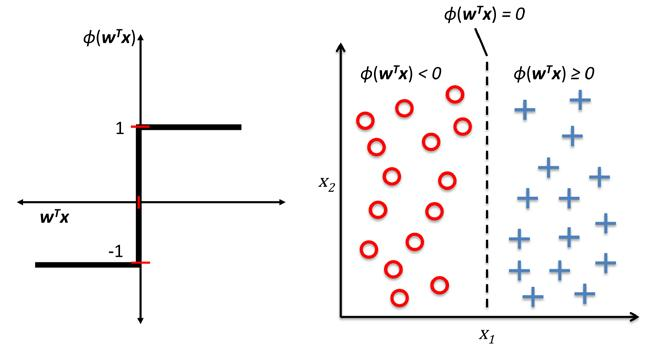
\includegraphics[scale=0.5]{perceptron} \centering
  \caption{\textit{Aplanamiento} de la salida del perceptrón para
    hacer clasificación.  (Tomado de \cite{python})}
  \label{fig:binary}
\end{figure}

La idea detrás del modelo de perceptron de Rosenblatt es reducir a una
abstracción de cómo funciona una neurona: se activa o no se
activa. Así, la regla inicial de Roseblatt es relativamente simple y
puede ser resumida en los siguientes pasos:
\begin{enumerate}
  \item Inicializar los pesos en cero o en números aleatorios cercanos
    a cero.
  \item Para cada muestra de entrenamiento $x^{(i)}$ realizar los
    siguientes pasos:
  \begin{enumerate}
    \item Calcular el valor de salida $\hat y$.
    \item Actualizar los pesos.
  \end{enumerate}
\end{enumerate}


En este caso, el valor de salida es la clasificación dada por la
función escalón definida previamente, y la actualización simultánea de
cada peso $w_j$ en el vector de pesos $w$ puede ser escrito más
formalmente cómo:
\begin{equation}
  w_j := w_j + \Delta w_j
\end{equation}

El valor de $\Delta w_j$, que es usado para actualizar el peso $w_j$,
es calculado por la regla de aprendizaje de percetron:
\begin{equation}
  \Delta w_j = \eta (y^{(i)} - \hat y^{(i)})x^{(i)}_j
\end{equation}

Donde $\eta$ es el índice de aprendizaje (una constante entre 0 y 1),
$y^{(i)}$ es la clasificación real de la i-ésima muestra, y $\hat
y^{(i)}$ es la clasificación dada por la predicción. Es importante
recalcar que todos los pesos en el vector de pesos son actualizados de
manera simultánea, lo que significa que no recalculamos $\hat y^{(i)}$
hasta que todos los pesos $\Delta w_j$ han sido actualizados.

\begin{figure}[H]
  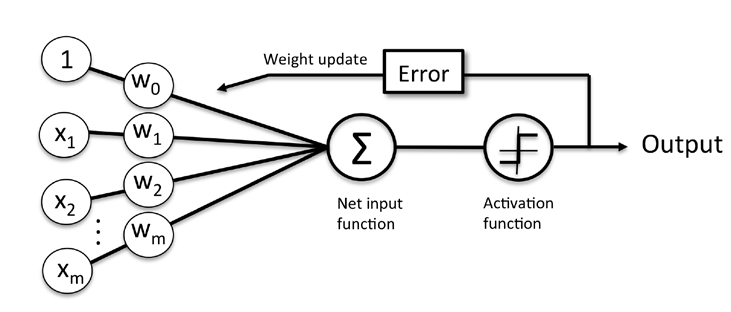
\includegraphics[scale=0.5]{perceptron-summary} \centering
  \caption{Resumen del concepto general de perceptrón. (Tomado de
    \cite{python})}
  \label{fig:perceptron}
\end{figure}

La figura \ref{fig:perceptron} muestra cómo el perceptron recibe las
entradas de una muestra $x$ y las combina con los pesos $w$ para
calcular la entrada neta.  Esta entrada se le da a la función de
activación, que genera una salida binaria (-1 o 1 en este caso),
representando la predicción de la clasifica- ción. Durante la fase de
aprendizaje, la salida es usada para calcular el error de la
predicción y actualizar los pesos.

\section{Neuronas adaptativas lineales}

\begin{figure}[H]
  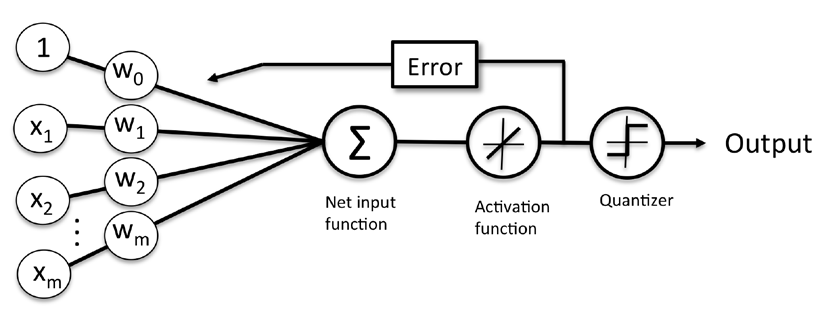
\includegraphics[scale=0.5]{adaline} \centering
  \caption{Esquema de Adaline. (Tomado de \cite{python})}
  \label{fig:adaline}
\end{figure}

La neurona adaptativa lineal (\textbf{Adaline}) fué publicada unos
años después del algoritmo del perceptrón de Frank Rosenblatt, por
Bernard Widrow \cite{adaline} y se considera la evolución natural del
perceptrón de Rosenblatt.  El algoritmo de Adaline es particularmente
interesante porque ilustra el concepto clave de definir y minimizar
funciones de costo, lo que sienta las bases para algoritmos mas
avanzados de clasificación, como la regresión logística o las máquinas
de vectores de apoyo.

La principal diferencia entre las reglas de Adaline (también llamada
de \textit{Widrow-Hoff}) y la del perceptrón de Rosenblatt es que los
pesos son actualizados con base en una función de activación lineal,
en lugar de una función escalón. En Adaline, esta función de
activación $\phi (z)$ es simplemente la función identidad de la
entrada neta, así $\phi (w^T x) = w^T x$.

Mientras que la función de activación lineal es usada para la
actualiza- ción de pesos, un \textit{cuantificador}, similar a la
función escalón descrita anteriormente, puede ser usado para hacer la
clasificación, como se ilustra en la figura \ref{fig:adaline}.

Si se compara la figura \ref{fig:perceptron} con la figura
\ref{fig:adaline}, la diferencia es que se usa la salida con valores
continuos de la función lineal de activación para calcular el error y
actualizar los pesos, en lugar de hacer una clasificación binaria.

Cabe destacar que actualmente se buscan funciones de activación más
suavizadas y, sobre todo, diferenciables. Esto con el fin de optimizar
los parámetros de los modelos más complejos.

\begin{figure}[H]
  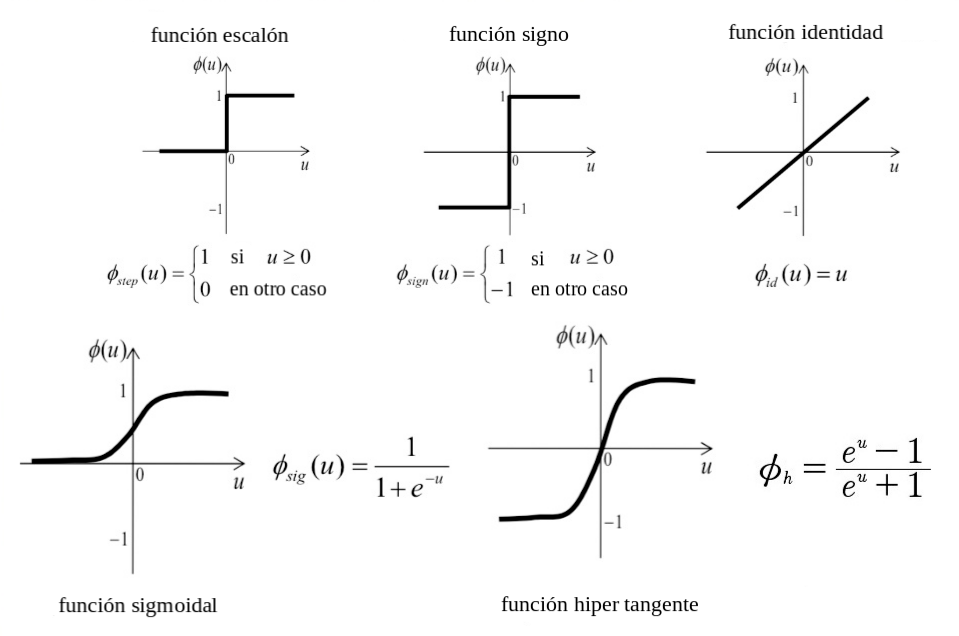
\includegraphics[scale=0.5]{activation} \centering
  \caption{Algunos ejemplos de otras funciones de activación.  (Tomado
    de
    \url{https://www.slideshare.net/SungJuKim2/multi-layer-perceptron-back-propagation})}
\end{figure}

\section{El perceptrón multicapa}
El perceptrón multicapa es una generalización del perceptrón simple de
Rosenblatt, como conescuencia de las limitaciones de este ante
conjuntos de datos que no son linealmente separables. Lo que se hace
es combinar varios perceptrones en una \textit{red neuronal de
  propagación hacia adelante}, con una estructura de \textit{capas}.

La información fluye de capa en capa en el mismo sentido, desde la
\textit{capa de entrada} donde están los datos sin procesar, hasta la
\textit{capa de salida} dónde se da la clasificación. Cada capa
intermedia, llamadas \textit{capas ocultas}, consta de un conjunto de
neuronas sin conexiones entre ellas, pero totalmente conectadas a las
capas inmediatamente anterior y posterior. Visto como una gráfica, un
\textbf{perceptrón multicapa} (\textit{MLP} por sus siglas en inglés)
es una gráfica $n-partita$ dirigida donde $n$ seria el número de
capas.
\begin{figure}[H]
  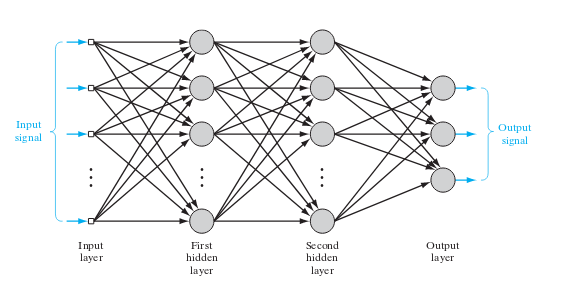
\includegraphics[scale=0.5]{mlp} \centering
  \caption{Arquitectura de un MLP con dos capas ocultas (Tomado
    \cite{haykin})}
\end{figure}
Cada neurona oculta actua como un \textit{detector de
  características}. Conforme va avanzando el proceso de aprendizaje,
las neuronas ocultas comienzan a ``descubrir'' gradualmente las
características más sobresalientes de los datos de entrenamiento.
Esto se logra a través de una serie de transformaciones no lineales,
dadas por las funciones de activación y pesos específicos de cada
neurona.

Inicialmente, a cada neurona se le asigna un peso aleatorio. Dada la
estructura en capas de la red, es mucho más fácil visualizar y
manipular estos pesos acomodandolos en una matriz $W$, que llamaremos
\textit{matriz de pesos}, donde $W_i$ son los pesos de la $i$-ésima
capa de la red. Entonces, dado un vector de entrada $x$, la primera
capa oculta $h_1$ calcula su valor a partir de $W_1$ y una traslación
$b_1$, que llamamos \textit{sesgo} (en inglés, \textit{bias}), del
siguiente modo:
\begin{equation}
  h_1 = \sigma(W_1x + b_1)
\end{equation}
donde $\sigma$ es una función de activación no lineal y
diferenciable. Así la $i+1$-ésima capa oculta computa su valor como
\begin{equation}
  h_{i+1} = \sigma(W_{i+1}h_i + b_{i+1})
\end{equation}
Por último, la salida, suponiendo que hay $n$ capas ocultas, seria
\begin{equation}
  \hat{y} = \sigma{(W_{n+1}h_n + b_{n+1})}
\end{equation}
donde $\hat{y}$ es el vector de clasificación.
